\section{Введение}
Работа выполнена в лаборатории "Оптика сложных квантовых систем" Отделения Оптики
под руководством Ивана Кожокару. На первом занятии нам провели экскурсию по 
лабораториям -- показали квантовые компьютеры, атомные часы, резонаторы для
создания ультрастабильных лазерных систем, и,
собсвенно, лабораторию по изучению центров окраски. На следующем занятии 
именно в последней нам выдали задание: в лабораторию пришли образцы алмазных пластин
с внедрёнными центрами окраски, но производитель не указал, какие именно атомы 
внедрены в кристаллическую решётку. Нам предстояло это выяснить. 

Центры окраски в алмазах -- это атомы, внедрённые в кристаллическую решётку
алмаза. Наиболее интересными изученными центрами окраски являются NV-, GeV-
и SiV-центры. Уровни энергии электронов, связанных с этими центрами, имеют ряд
свойств, которые могут быть использованы в практических целях. Например, 
зависимость вида спектра люминесценции от температуры может быть основой для микроскопического
датчика температуры, который применяется в исследовании внутриклеточной активности
живых существ \cite{Therm}. Кроме того, такой датчик может быть использован
как замена существующих полупроводниковых термометров, в том числе в экстремальных
условиях. Алмаз с центрами окраски может быть использован для измерения магнитного
поля, что в перспективе открывает новые возможности для геологических исследований. 

Системы электронных уровней GeV-центров и SiV-центров имеют одинаковую структуру, см. рис.
\ref{Energy levels GeV}, \ref{Energy levels SiV}. NV-центры в данной работе не рассматриватся:
для использования их в качестве микроскопического датчика температуры требуется 
воздействие микроволного излучения, каковое не может быть сфокусировано на одну клетку и,
кроме того, может её разрушить \cite{Therm}. Основной переход $\gamma_r$ имеет 
длину волны $\lambda_{GeV} \approx 605 \text{ нм}$, $\lambda_{SiV} \approx 740 \text{ нм}$
соответственно у GeV и у SiV центров.

\begin{figure}[!h]
    \begin{center}
        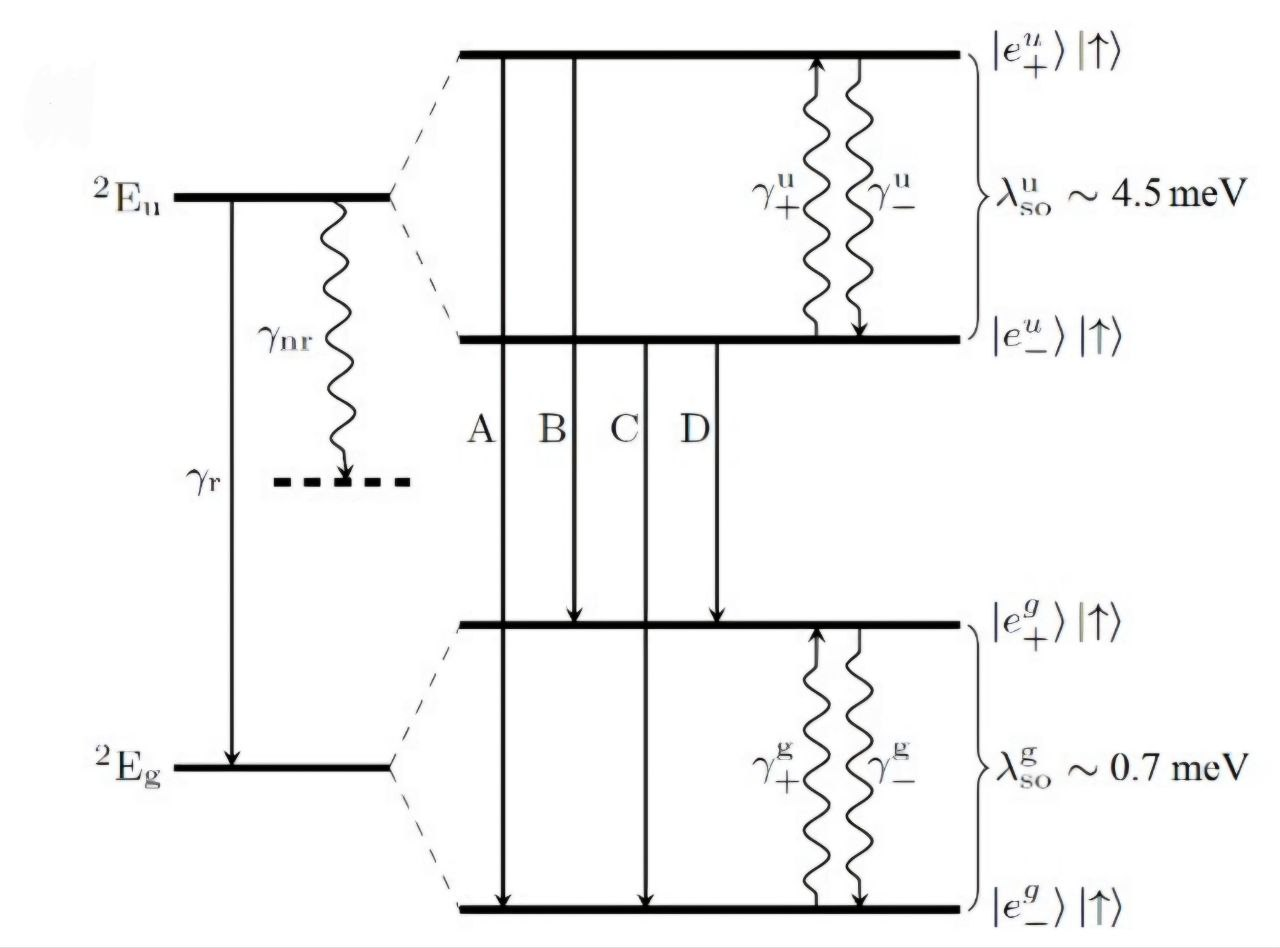
\includegraphics[width=0.7 \linewidth]{Energy levels GeV.jpg}
        \caption{Схема уровней оптического электронного перехода в GeV-центре.
        Сплошными прямыми линией отмечены оптические переходы,
        волнистыми -- нерадиационные переходы.}
        \label{Energy levels GeV}
    \end{center}
\end{figure}

\begin{figure}[!h]
    \begin{center}
        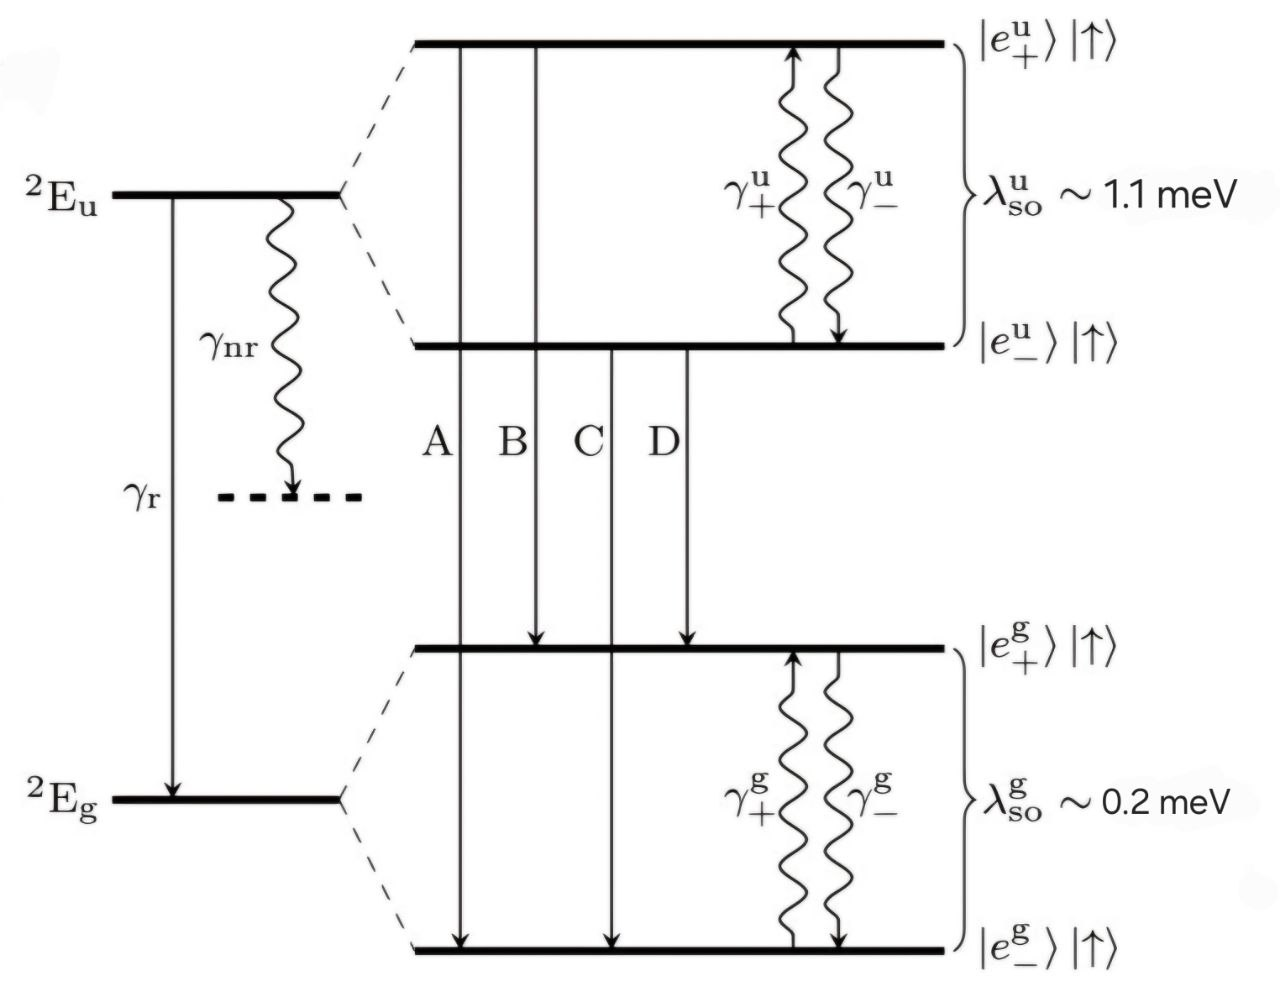
\includegraphics[width=0.7 \linewidth]{Energy levels SiV.jpg}
        \caption{Схема уровней оптического электронного перехода в SiV-центре.
        Сплошными прямыми линией отмечены оптические переходы,
        волнистыми -- нерадиационные переходы.}
        \label{Energy levels SiV}
    \end{center}
\end{figure}

Основной и первый возбуждённый уровни расщеплены на два вследствие
спин-орбитального взаимодействия: спин электронной оболочки $s_z$ = $\pm$1/2,
а момент импульса $l_z$ = $\pm$1. Каждый из этих уровней дважды вырожден.
При нулевой температуре можно наблюдать
4 линии (A, B, C и D на рис. \ref{Energy levels GeV}, \ref{Energy levels SiV}), 
однако при повышении температуры
происходит уширение линий вследствие эффекта Яна-Теллера, и линии тонких структур
перестают быть различимыми. Этот эффект
проявляется в поглощении или испускании фонона при переходе электрона между
подуровнями тонкой структуры. На рис. \ref{J-T effect} изображены возможные переходы электрона:
в случае (a) поглощается один фонон, соответствующий энергии перехода. В случаях
(b) и (c) поглощаются 2 фонона, имеющих такие энергии, чтобы их сумма была 
равна энергии перехода. В исследуемых центрах окраски процесс (b) не происходит.

Таким образом, приведённый эффект при известных константах позволяет определять 
температуру по ширине линии люминесценции. Кроме того, имеется зависимость 
положения пика люминесценции и расстояния между пиками от температуры. Одной из целей 
работы лаборатории является как можно более подробное исследование этих зависимостей для
получения возможности определения температуры алмаза.

\begin{figure}[!h]
    \begin{center}
        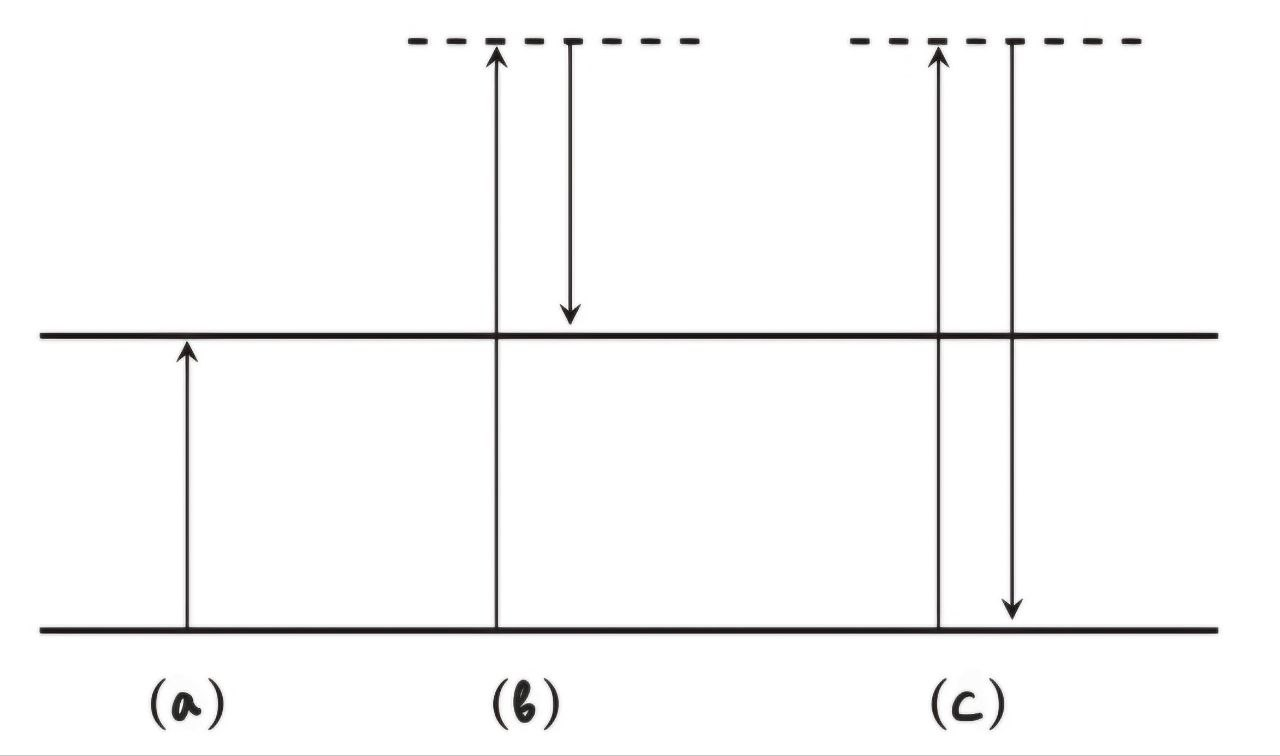
\includegraphics[width=0.5 \linewidth]{Jahn-Teller effect.jpg}
        \caption{(a) -- прямой однофононный процесс, (b) -- двухфононный
        Рамановский процесс, (c) -- упругое рассеяние фононов}
        \label{J-T effect}
    \end{center}
\end{figure}


